\documentclass[../main.tex]{subfiles}
\begin{document}

\chapter{Methods}
\labch{methods}

In this section I shall describe some general methods which are widely 
used in quantitative genetics and bioinformatics, and were also employed 
in the articles described in the thesis.

\section{Regression}
\labsec{regression}

Regression is used to find relationship between data. It usually 
consists of three-steps:

\begin{enumerate}
	\item Assumption-making, where one chooses the type of relationship 
(\eg linear, logistic, polynomial...).
	\item Fitting of the model, where the parameters of the model are 
evaluated on a training data set.
	\item Prediction of the response, where known data from a testing 
data set are fed to the model, which returns an estimation of the 
outcome.
\end{enumerate}

\newthought{Linear regression\autocite{James2013}} models a linear 
relationship between a continuous variable, $Y$, and one or more other 
variables, the $X$'s, which may be continuous or categorical. In other 
words, $Y$ can be expressed as

\begin{equation}
	Y \approx \beta_0 + \beta_1X_1 + \beta_2X_2 + \ldots + \beta_pX_p\,,
\end{equation}

where the $\beta$'s are called the model coefficients; the approximation 
sign is due to random errors, which causes the $Y$ to differ from the 
right-hand side by a term $\epsilon$ ---a random residual error. In 
simple linear regression, at first the model is fitted, \ie the values 
of the coefficients that better describe the relationship between $X$ 
and $Y$ are found relying on a training dataset, and the model is 
applied to a testing dataset with known $X$'s to make predictions of 
$Y$. The fitted model, where the parameters are estimated, is usually 
represented as follows, with the parameters denoted by an hat:

\begin{equation}
	\hat{y} = \hat{\beta}_0 + \sum_{j=1}^{p}\hat{\beta}_j x_j\,.
\end{equation}

The estimation of the coefficients is often made by the minimisation of 
the residual sum of squares, which is defined as 
$\sum_{i=1}^{n}(y_i~-~\hat{y_i})^2$, \textit{i.e.}\ 
$\sum_{i=1}^{n}(y_i~-~(\hat{\beta}_0~+~\sum_{j=1}^{p}\hat{\beta}_jx_j))^2$.

The coefficients are obtained by using some calculus to find the partial 
derivatives of the RSS function with respect to all the $\hat{\beta}$, 
and then some algebra to solve a $p$th-order linear system where we 
impose such derivatives equal to 0.

\marginnote{When $p=2$, the partial derivatives are
\begin{flalign*}
&\frac{\partial RSS}{\partial \hat{\beta}_0} =
	\sum_{i=1}^{n} -2 (y_i - \hat{\beta}_1 x_i - \hat{\beta}_0)
&\\
&\frac{\partial RSS}{\partial \hat{\beta}_1} =
	\sum_{i=1}^{n} -2 x_i (y_i - \hat{\beta}_1 x_i - \hat{\beta}_0)
\end{flalign*}
and the system yields
\begin{flalign*}
&\hat{\beta}_0 = \bar{y} - \hat{\beta}_1\bar{x}
&\\
&\hat{\beta}_1 = \frac{\sum_{i=1}^{n}(x_i - \bar{x})(y_i - \bar{y})}
	{\sum_{i=1}^{n}(x_i - \bar{x})^2}
\end{flalign*}
}

Once we have the coefficients, given the $x$'s, we could estimate an 
$\hat{y}$.

\newthought{Ridge regression\autocite{James2013}}, which is similar to 
linear regression, is a regularisation method which allows to reduce the 
dependance of the fitting on the training set of values by shrinking the 
coefficients towards zero. This is achieved with a slight modification 
of the least squares, that is, the function to minimise is

\begin{equation}
	\sum_{i=1}^{n}\left(y_i-\beta_0-\sum_{j=1}^{p}\beta_jx_{ij}\right)^2+
		\lambda\sum_{j=1}^{p}\beta_j^2\,.
\end{equation}

This function is the sum of the RSS and a penalty term, the minimisation 
of which can improve the fitting of the model, provided that the tuning 
parameter $\lambda$ is properly chosen.

\newthought{The lasso\autocite{Tibshirani1996}} is another regularisation 
method which allows to effectively select a subset of relevant 
predictors by setting the coefficients of the others to zero. In this 
case, the minimisation function is

\begin{equation}
	\sum_{i=1}^{n}\left(y_i-\beta_0-\sum_{j=1}^{p}\beta_jx_{ij}\right)^2+
		\lambda\sum_{j=1}^{p}\left|\beta_j\right|\,.
\end{equation}

\newthought{Elastic net\autocite{Zou2005}} combines the best features of 
ridge regression and lasso by introducing two penalty terms:

\begin{equation}
	\sum_{i=1}^{n}\left(y_i-\beta_0-\sum_{j=1}^{p}\beta_jx_{ij}\right)^2+
		\alpha\sum_{j=1}^{p}\left(\beta_j\right)^2+
		(1-\alpha)\sum_{j=1}^{p}\left|\beta_j\right|\,,
\end{equation}

with $\alpha$ between 0 and 1. Its main advantage is that it works well 
when $p>n$, for it can potentially group correlated predictors and 
select only one representative variable for each group.

Elastic net is used in the paper by Gamazon \etal (\refch{gamazon2015}) 
to predict the genetically regulated component of gene expression.

\newthought{Logistic regression\autocite{James2013}}, which applies when the 
predicted outcome is a binary variable indicating whether the response 
falls into one of two categories, models the probability that the 
variable belongs to a particular category.

While for linear regression we assumed an equation of the form of a 
straight line (or a multi-dimensional equivalent), for logistic 
regression we need a function that returns values between 0 and 1, thus 
we rely on the logistic function (\reffig{logistic}):

\begin{equation}
	Y = P(Z = 1 | X) =
		\frac{\exp(\beta_0+\beta_1X)}{1+\exp(\beta_0+\beta_1X)}\,.
\end{equation}

\begin{marginfigure}
	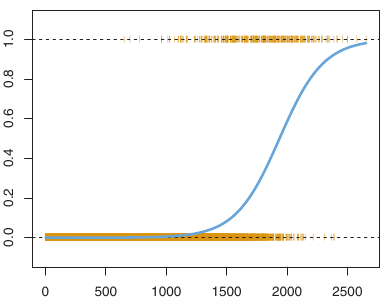
\includegraphics{methods/logistic}
	\caption{An example of logistic model. Adapted from \textcite{James2013}}
	\labfig{logistic}
\end{marginfigure}

In order to fit this model we switch to the \enquote{estimated} values, 
denoted by an hat, and manipulate the logistic function until we have

\begin{equation}
	\log\left(\frac{\hat{y}}{1-\hat{y}}\right) =
		\hat{\beta}_0 + \hat{\beta}_1 x\,,
\end{equation}

where the left-hand member is the logarithm of the odds, or logit. At 
this point the coefficients can be found with the maximum likelihood 
method, and the predictions be made. As with linear regression, this 
model can be easily extended to include more than one predictor.

Logistic regression is used in Gamazon \etal to find the probability of 
disease given the expression level of a gene.

\newthought{Linear mixed models} are useful when data have an 
hierarchical structure, \ie there can be identified many groups and 
there is variability both inside and among groups. Such models cobine 
fixed and random effects as predictors of the outcome. The relationship 
between the predictors and the outcome is as follows.

\begin{equation}
	Y = \beta_0 + \sum_{j=1}^{p} \beta_j X_j +
		u_0 + \sum_{j=1}^{q} u_j Z_j + \epsilon
\end{equation}

The $X$'s are the predictor variables, with the $\beta$'s as their 
coefficients; the $uZ$'s are the random effects, random because the 
$u$'s are assumed to be normally distributed; and $\epsilon$ is the 
residual random error.

\newthought{A bayesian sparse linear mixed model\autocite{Zhou2013a}} is 
a linear mixed model because the outcome depends on both fixed and 
random effects, is sparse because it selects only a subset of all the 
predictors (like the lasso or elastic net), and is Bayesian because the 
predictors are selected using a Bayesian approach.

One of these models is used in both papers by Gusev \etal 
(\refch{gusev2016}, \refch{gusev2018}) to predict the expression levels 
of genes in a reference transcriptome data set.

\section{eQTL mapping}
\labsec{eqtl}

There are many ways to perfom an eQTL analysis\autocite{Gilad2008}, but the 
underlying idea is that of considering gene expression as a quantitative 
trait and finding associations between a genetic variant and this 
phenotype. The association, which can exist both for \cis and for \trans 
variants, can be found either through correlating genotype and 
expression, or by using a linear regression model for each gene-marker 
pair between the number of alleles that individuals have at the marker 
locus and the expression of the gene.

\begin{figure}
	\centering
	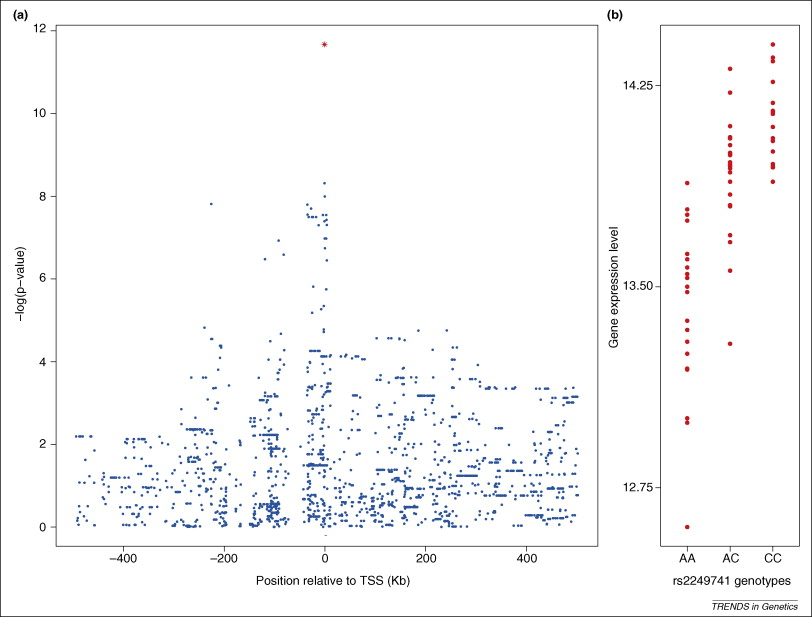
\includegraphics[width=0.8\textwidth]{methods/eQTL}
	\caption{Typical eQTL results.}
	\labfig{eqtl}
\end{figure}

\section{GWAS}
\labsec{gwas}

To perform a genome-wide association study\autocite{Clarke2011}, two 
types of data about the individuals are needed: genetic markers and 
phenotypes. For each individual, its two alleles at each of the loci 
under study are reported; such loci are called markers, because they 
mark a specific position on a chromosome. Phenotypic data is needed to 
split the population in cases and controls, and possibly to detect and 
correct false associations: indeed, differences in the allele 
frequencies of cases and controls could be due to differences in sex, 
population stratification or other conditions that differ from cases to 
controls. Since only a few loci are typed in a normal GWAS, it is often 
performed an imputation step, where SNPs at other loci are estimated on 
the basis of their LD structure.

After making quality controls and corrections for causes of variance not 
due to the phenotype of interest (\ie, covariates, which are a possible 
source of confounding), the frequency of each allele at each marker in 
cases and controls is computed. At this point, there are a few choices 
about how to perform the test of association. The simplest model is 
based on allele counts.

First of all, a contingency table like that in \reftab{gwas_contingency} 
is built.

\begin{table}
	\centering
	\begin{tabular}{ l c c l}
		\toprule
		Allele & a & A & Total \\
		\midrule
		Cases & $m_{11}$ & $m_{12}$ & $m_{1\cdot}$ \\
		Controls & $m_{21}$ & $m_{22}$ & $m_{2\cdot}$ \\
		Total & $m_{\cdot1}$ & $m_{\cdot2}$ & $2n$ \\
		\bottomrule
	\end{tabular}
	\caption{Contingency table for an allelic model of association.}
	\labtab{gwas_contingency}
\end{table}

The odds ratio for allele A is estimated by

\begin{equation}
	OR_A = \frac{\frac{m_{12}}{m_{11}}}{\frac{m_{22}}{m_{21}}} =
		\frac{m_{12}m_{21}}{m_{22}m_{11}}
\end{equation}

And the association test is actually a $\chi^2$ test of independence of 
rows and columns, the significance threshold of which should be 
corrected for the multiple testing performed at each marker.

\begin{equation}
	\chi^2 = \sum_{i=1}^{2} \sum_{j=1}^{2}
		\frac{(m_{ij} - E[m_{ij}])^2}{E[m_{ij}]}
\end{equation}

\end{document}
